\documentclass[11pt,a4paper]{article}
\usepackage[latin1]{inputenc}
\usepackage{amsmath}
\usepackage{enumerate}
\usepackage{breakcites}
\setlength{\parindent}{0pt}
\usepackage[scale=0.8]{geometry}
\usepackage{amsfonts}
\usepackage[hidelinks]{hyperref}
\usepackage{amssymb}
\usepackage{makeidx}
\usepackage{lscape} %for switching between landscape and portrait
\usepackage{graphicx}
\author{James Mba Azam}
\title{Modelling Hepatitis B Mother-to-Child Transmission in sub-Saharan Africa - A Focus on the
	Impact of Vaccination Within Existing HIV MTCT Infrastructure.}
\begin{document}
	
\title{\textbf{Modelling Hepatitis B Vertical Transmission in sub-Saharan Africa - A Focus on the
		Impact of Birth Vaccination on Possible Eradication.}}
\date{\today}
\author{James Mba Azam\\ (Department of Mathematical Sciences, Stellenbosch University \& SACEMA)\\Supervisors: Prof. Martin Nieuwoudt, Dr. Eben du Toit, Dr. Monique Ingrid Andersson}
\maketitle
%\section{Introduction}
%Not much work has been done on the analysis of vertically-transmitted diseases and the paper \cite{busenberg1982models} affirms this fact.
%\section{Introduction}
\subsection{Aim}
To mathematically ascertain whether  hepatitis B eradication is possible in the near future by focusing on preventing vertical transmission of the infection. 
\subsection{Research Questions}
To achieve the stated aim, this research  will try to answer the following question: Can Hepatitis B be eradicated from Sub-Saharan Africa (SSA) within a couple of generations, given the intervention is limited to preventing vertical transmission by administering an extra dose of vaccine at birth to the neonates, as well as treating infected mothers and their babies?


%\subsection{Research Questions}
%To achieve the aim stated above, this research  will try to answer the following question and sub-questions: \label{section: research question}Can Hepatitis B be eradicated from Sub-Saharan Africa (SSA) within a couple of generations, given the intervention is limited to: 
%\begin{enumerate}[(a)] 
%	\item MTCT (mother-to-child-transmission)?,
%	\item the child (either/or/neither/nor/both/none)?
%	\item Established rates and prevalences of  HBV in SSA?
%\end{enumerate}

\subsection{Objectives}
In this research, we seek to:
\begin{enumerate}
	\item Propose a novel deterministic SIR type model for vertical transmission which captures interventions applied to both the mothers and their newborns.
	\item Check whether the interventions introduced in the model affects the population dynamics of the infected infants.
	\item Ascertain the contribution of the infected infants to the disease dynamics in the general population.
	\item Study the possibility of eradication by following up the results in the previous objectives stated.
	%\item Given data on pregnant women in SSA, find or estimate rates/measures of risk for HBV MTCT.
\end{enumerate}
\subsection{Approach/Methods}
The model will have two ``stages":
\begin{itemize}
	\item 	Stage 1: The intervention(s) applied to mothers and their babies in primary health-care settings. 
	\item Stage 2: The model from Stage 1 will have the output called ``children born with HBV infection". 
\end{itemize} 
This output will flow into a larger SSA birth/death model for simulation over generations.  
The total contribution of HBV+ children into the larger population will thus be the foundation
on which the hypothesis of eradication will be shown in this work.
\section{Preventing Hepatitis B Mother-to-Child Transmission}
	Many countries are prioritizing the hepatitis B eradication. Several articles for instance: \cite{andersson2015mother, xu2013nextstep,tran2009management,shimakawa2016mother} have posited that we will have to concentrate on preventing the mother-to-child transmission route if this is to be achieved in the near future. The paper \cite{Pan2012} did a review of articles published between 1975-2011 on HBV mother-to-child transmission and deduced that by administering Hb immunoglobulin alongside the Hb vaccine between the time of birth and at most 12 hours after exposure, combined with administering the existing vaccination regimen between 6-12 months to an infant, it will provide an approximate 95\% chance of preventing the perinatal transmission of HBV from their HBsAg-positive pregnant mother. Concerning the use of tenofovir as immunoprophylaxis for reducing HBV MTCT, a very recent study in the paper \cite{pan2016tenofovirToPrevent} has corroborated that it might be a better and possibly, safer option in the near future, as predicted by the authors in \cite{xu2013nextstep}. More importantly, it has been been suggested that the second dose must be administered in a very timely fashion, as a study by \cite{tharmaphornpilas2009increasedRisk} has proven that a delay in the subsequent vaccines could prove to be a hindrance in protecting the infants against the transmission of HBV.
	
	\section{HBV Mother-to-Child Transmission Risk Factors}
	According to  \cite{Pan2012}, an efficient way to prevent MTCT of HBV is to assess the risk of MTCT, and to identify the mothers who possessed the most risk so as to administer the interventions to prevent MTCT. Eventually, they listed: maternal level of HBV DNA $>200,000$ IU/mL, positive test(s) for the HB envelope Antigen(HBeAg) and HB surface Antigen(HBsAg), pregnancy complications such as threatened pretem labour, or prolonged labour, and failure of the immunoprophylaxis in children who had received it, as the risk factors to consider. For simplicity, the model in this document will consider the following risk factors stemming from those listed in the paper \cite{Pan2012}: HBV DNA of pregnant women greater than $200,000$IU/mL, and pregnant women who are both HBeAg and HBsAg positive. 

	
	\section{Assumptions of the Model}
	\begin{enumerate}
	\item Infants below one year do not die of hepatitis b related causes.
	\item no horizontal transmission in infants.
	\item The intervention provides $95\%$ efficacy.
	\item Only infected mothers and those on treatment may produce infected babies. 
	\end{enumerate}
		
	\section{Model Framework}
		The model flowchart was generated by linking up three interacting models of two types: $SVVPIT$ for neonates of age-class $b1$, and $SVPIT$ for infants of age-class $b2$ and pregnant adult females of category $m$.
		
		The model consists of the following class of individuals: susceptible individuals $(S_m)$, $(S_{b1})$ and $(S_{b2})$, infants who have received their first dose at birth or within 24 hours $(V_{b1})$, and infants who have received their full dosage of the current vaccine regimen $(V_{b2})$. It is worth noting that the class $V_{b2}$ contains neonates who were vaccinated at birth and those who were not, so far as they remained uninfected. The other classes are: fully protected individuals $(P)$, infected individuals $(I)$, a class of individuals who have been treated, or are under treatment $(T)$.
		
		\subsection{Flowchart Description}
		Neonates are either born infected or uninfected and that is how $S_{b1}$ and $I_{b_1}$ are populated. Some of these individuals receive their first dose immediately after birth, moving to $V_{b1}$. Since it is assumed the first dose does not provide full protection, some of the vaccinated neonates may be infected before they receive the second set of vaccines; those individuals populate $I_{b1}$ alongside those infants who get infected because they were not vaccinated. Since the vaccine may wane off, some of the vaccinated individuals in $V_{b1}$ may become 
		
		The flow chart is represented in Figure \ref{fig:flowchart}. The equations will be generated subsequently upon discussing the flow diagram and after all necessary inputs have been implemented and approved.
		\begin{figure}[h!]
			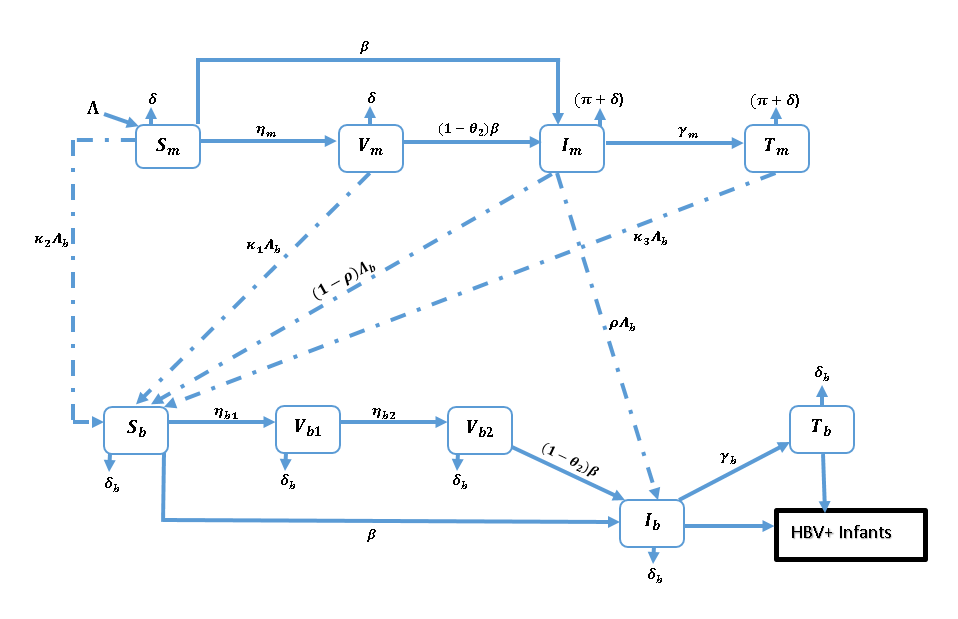
\includegraphics[scale=0.7]{new_model}
			\caption{Shows the model structure indicating vertical and horizontal transmission. The solid arrows indicate movement of the individuals, and the dashed arrows represent births.} \label{fig:flowchart}
		\end{figure}
		\newpage
	\subsection{Description of State Variables and Parameters}
%	The individuals were split into three age classes and represented as follows:
%	\begin{itemize}
%		\item $m$ refers to pregnant women (of at least their average age to be determined from the data).
%		\item $b1$ represents neonates of less than age 1 day.
%		\item $b2$ is used to denote neonates older than 1 day but less than the average age of the pregnant women(to be obtained from the data).
%	\end{itemize}
	The following are the variables and parameters used so far:\vspace{1.5mm}
	
	$S_{b1}$: Susceptible neonates below age 1 day \vspace{1.5mm}
	
	$S_{b2}$: Susceptible neonates older than age 1 day without a first dose at birth\vspace{1.5mm}
	
	$S_{m}$: Susceptible pregnant women\vspace{1.5mm}
	
	$V_{b1}$: Vaccinated neonates at time of birth\vspace{1.5mm}
	
	$V_{b2}$: Vaccinated infants with or without a first dose at birth but of the age-class $b2$\vspace{1.5mm}
	
	$V_{m}$: Vaccinated pregnant mothers\vspace{1.5mm}
	
	$P$   : Protected individuals (refer to assumptions for details)\vspace{1.5mm}
	
	$V_{m}$: Vaccinated pregnant women\vspace{1.5mm}
	
	$I_{b1}$: Infected neonates below 1 day old \vspace{1.5mm}
	
	$I_{b2}$: Infected neonates older than 1 day but at most, a year old. \vspace{1.5mm}
	
	$I_{m}$: Infected pregnant women\vspace{1.5mm}
	
	$T_{b1}$: Neonates below age 1 day and are under treatment\vspace{1.5mm}
	
	$T_{b2}$: Infants older than 1 day old, but at most, a year old, and under treatment \vspace{1.5mm}
	
	$T_{m}$: Pregnant women under treatment.\vspace{1.5mm}
	
	$\pi_0$: Natural death rate (assumed to be the same across ages)\vspace{1.5mm}
	
	$\pi_b$: Infant mortality rate\vspace{1.5mm}
	
	$\pi_h$: hepatitis b related death rate\vspace{1.5mm}
		
	$\mu_b$: Birth rate \vspace{1.5mm}
	
	$\rho$: Proportion born uninfected\vspace{1.5mm}
	
	$\phi_1$: Proportion of susceptible infants who are female and become pregnant\vspace{1.5mm}
	
	$\phi_2$: Proportion of infected infants who are female and become pregnant\vspace{1.5mm}
	
	$\phi_3$: Proportion of treated infants who are female and become pregnant\vspace{1.5mm}
	
	$\kappa_1$: Proportion of $b1$ neonates who remain susceptible till $b2$ \vspace{1.5mm}
	
	$\kappa_2$: Proportion of $b1$ neonates who remain infected till $b2$ \vspace{1.5mm}
		
	$\kappa_3$: Proportion of $b1$ neonates who remain under treatment till $b2$ \vspace{1.5mm}
	
	$\theta_1$: Efficacy of the first dose  of vaccine at birth  \vspace{1.5mm}
	
	$\theta_2$: Efficacy of the current vaccine regimen \vspace{1.5mm}
	
	$\beta$: Rate of infection \vspace{1.5mm}
	
	$\alpha_1$: Rate of waning of the first vaccine \vspace{1.5mm}
	
	$\alpha_2$: Rate of waning of the current vaccine regimen \vspace{1.5mm}
	
	$\lambda$: Rate of acquiring antibodies \vspace{1.5mm}
	
	$\gamma_{b1}$: Treatment rate of infected $b1$ neonates \vspace{1.5mm}
	
	$\gamma_{b2}$: rate of treatment of the infected $b2$ neonates \vspace{1.5mm}
	
	$\gamma_{m}$: Treatment rate of infected pregnant women \vspace{1.5mm}
	
	$\eta_{b1}$: vaccination rate of infants at the point of birth \vspace{1.5mm}

	$\eta_{b1}^*$: rate of second vaccination, after the dose at birth \vspace{1.5mm}	
	
	$\eta_{b2}$: vaccination rate of infants classified under $b2$ on the current regimen\vspace{1.5mm}
		
	$\eta_{m}$: rate of vaccinating the pregnant nothers\vspace{1.5mm}
	
	
	
	
		
	
	
	
	
	

	
	
	
	
	
	
	
	
	
	
	
	
	\newpage
	\bibliographystyle{apalike}
	\bibliography{refs}
\end{document}